\scanpage{44}
Revenons aux conditions de la \uline{proposition}, et déterminons
\[
\omega_{G_0}=t_{G_0}^{\vee}\simeq M_\nu/\unsure{\pi^F|\pi}M_\nu\simeq\Omega/p\Omega
\]
avec $k=A/\pi A$ y opérant de la façon évidente, et la structure de vectoriel sur \inserted{$W/pW=$} $k=\mathbb F_q$ est déduite de la structure précédente grâce à $\sigma^\nu$. Le cas le plus simple est celui où $\nu=0$, i.e. où \deleted{\unsure{les deux}} les deux opérations de $k$ sur $\omega_{G_0}$ coïncident. \deleted{\unsure{Si on a}} \unsure{Les autres|Ces autres} cas s'en déduisent grâce à \unsure{autom.} $\sigma^\nu$ de $k=\mathbb F_q$ \deleted{\unsure{$\sigma^\nu$}}).
\inserted{La filtration canonique sur $M\otimes_W k=\sum M_\nu\otimes_A k$ donne comme sous-module (de rg $1$) \deleted{\unsure{$M_0\otimes_A k$}} $\omega_0$ tel que $\unsure{\omega_0^{(p)}}\subset(M\otimes_W k)^{(p)}$ soit $\unsure{M_{f-1}\otimes_A k}$, i.e. qui donne $\omega_0=M_0\otimes_A k$.}

Le cas standart est
\[
G_0=G_0(A,\pi)\quad\text{correspondant à }(\nu=0\text{ et })\ \Omega=A
\]
on en déduit le cas d'un $\Omega$ quelconque par
\[
\deleted{\unsure{G_0}}\quad\Omega\otimes_A G_0(A)
\]
Donc on a dans ce cas comme module de Dieudonné
\[
\begin{cases}
M=A\otimes_{\mathbb Z_p}W\\
F_M=\mathrm{id}_A\otimes_{\mathbb Z_p}\sigma+\mathrm{pr}_0((\pi-1)\otimes\sigma)
\end{cases}
\]
où $\mathrm{pr}_0$ est la projection sur la composante correspondant au $A$-hom $A\otimes_{\mathbb Z_p}W\longrightarrow A$ qui sur $W$ est l'inclusion $W\overset{i}{\hookrightarrow}A$.

\figure{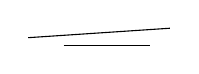
\begin{tikzpicture}
\draw (0,0)--(1.8,.12);
\draw (.45,-.10)--(1.55,-.10);
\end{tikzpicture}}

Nous nous proposons maintenant de relever $G_0$ \deleted{l'action} en un groupe de BT $G$ sur $A$, avec action de $A$ sur $G$, de telle façon que l'action \inserted{can.} de $A$ sur $t_G$ (qui est un $A$-module inversible) soit l'action évidente. D'après Lubin Tate,
\mspage{43}
